\documentclass[a4paper,french]{paper}
\usepackage{../../../../../_assets/latex/5N_OPTO_ELEC}

%Informations about this document 
%------------------------------------------
\def\module{Opto-Electronique - S5}
\def\moduleAbrege{5N-027-SCI / OptoElec}
\def\annee{2024-2025}

\def\titre{Séance 4 / Diodes}
\author{Julien VILLEMEJANE}

\subtitle{Séance 4}
\institution{LEnsE / Institut d'Optique Graduate School}

\title{\titre}
\begin{document} 
%Beginning First Page. 
%------------------------------------------
\enteteThematiqueObligatoire{}

\textit{Pour ce TD, on pourra s'appuyer sur la fiche résumée} : \href{https://lense.institutoptique.fr/ressources/Annee1/Electronique/fiches/2020_FR_Diodes_LED.pdf}{Diodes / LED / Photodiodes}

%Beginning Content. 

%%%%%%%%%%%%%%%%%%%
%%%%%%%%%%%%%%%%%%%
\encadreTDExo{4.1 - Limiter une tension}{
Rappeler le fonctionnement d'une diode.

Décrire le fonctionnement du montage suivant :

\begin{center}
\begin{circuitikz}
	\draw (0,0) to[battery2, invert] (0,5) to[short, -] (6,5)
		to[full diode=$D_1$, invert, i<_=$i_1$	] (6,2.5) to[full diode=$D_2$, invert, i<_=$i_2$, *-] (6,0)
		to[short, -*] (3,0) node[ground](GND){} to[short, -] (0,0);
	\draw (3,0) to[sV] (3,2.5) to[R=$R_p$, i=$i_R$] (6,2.5);
	\draw (6,2.5) to[short, -o] (8,2.5);
	\draw (8, 0) to[short, -o] ++(0,0) node[ground](GND){};
	\draw (8,0.3) edge[->,color={red}] (8, 2.2);
	\node[text={red}] (Vs) at (8.5,1.3){$V_S$}; 
	\draw (7,0.3) edge[<-,color={blue}] (7, 2.2);
	\node[text={blue}] (Vd2) at (7.5,1.3){$V_{D2}$}; 
	\draw (7,4.7) edge[->,color={blue}] (7, 2.8);
	\node[text={blue}] (Vd1) at (7.5,3.7){$V_{D1}$}; 
	\draw (2.5,0.3) edge[->,color={green!40!black}] (2.5, 2.2);
	\node[text={green!40!black}] (Ve) at (2,1.3){$V_e$}; 
	\draw (0.7,0.3) edge[->,color={black}] (0.7, 4.7);
	\node[text={black}] (Vcc) at (1.3, 2.5){$V_{CC}$}; 
\end{circuitikz}
\end{center}

}

%%%%%%%%%%%%%%%%%%%
%%%%%%%%%%%%%%%%%%%
\encadreTDExo{4.2 - Réguler une tension}{
Soit le montage suivant : 
 
 
\begin{center}
\begin{circuitikz}
	\draw (0,0) node[ground]{} 
		to[empty Zener diode=$D_Z$, i=$i_d$, -*] (0,2.5)
		to[R=$R_0$, i<_=$i_0$] (0,5)
		to[short, -] (-2,5)
		to[battery2] (-2,0)
		to[short,-*] (0,0);
	\draw[dashed] (0,2.5) to[short, -o, i=$i_s$] (2,2.5);
	\draw[dashed] (0,0) to[short, -o] (2,0);
	\draw (2,0.3) edge[<-,color={blue}] (2, 2.2);
	\node[text={blue}] (Vd) at (2.5,1.2){$u_d$};
	\draw (3,0.3) edge[->,color={red}] (3, 2.2);
	\node[text={red}] (Vs) at (3.5,1.2){$V_S$};
	\draw (-1.5,0.3) edge[->,color={black}] (-1.5, 4.7);
	\node[text={black}] (Vcc) at (-1,2.5){$V_{CC}$};
\end{circuitikz}
\end{center}

On donne une partie de la documentation d'une diode Zener de type 1N47xxA.

Expliquez le rôle de ce montage.

}

%%%%%%%%%%%%%%%%%%%
%%%%%%%%%%%%%%%%%%%
\encadreTDExo{4.3 - Redresser une tension}{

Soient les circuits suivants :

\begin{center}
	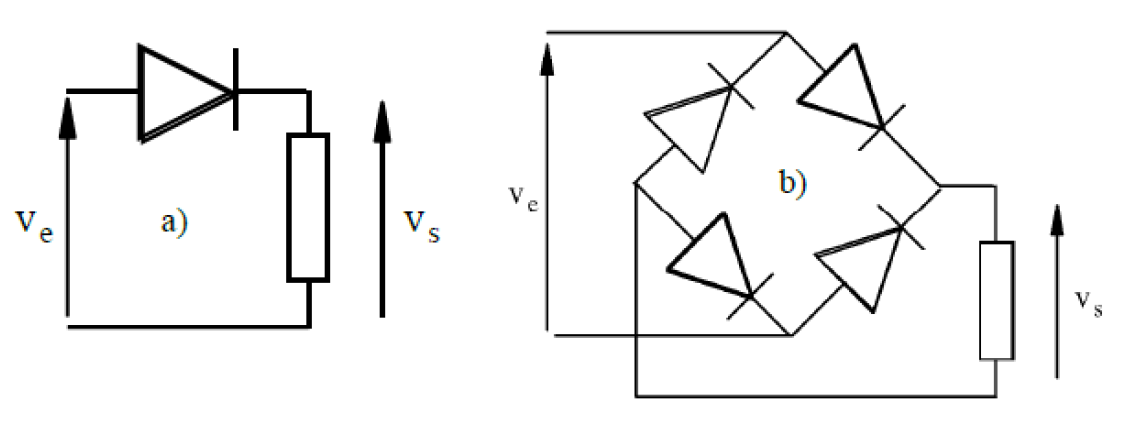
\includegraphics[width=8cm]{images/redresseur_001_a.png}
\end{center}

Donnez l'allure du signal de sortie $V_S(t)$ des circuits a et b suivants pour un signal d'entrée de forme sinusoïdale telle que $V_e(t) = A \cdot sin(\omega{}t)$ dans le cas d'une diode idéale. Puis dans le cas d'une diode avec une tension de seuil $V_d$. On supposera que $A > V_d$.

}

%%%%%%%%%%%%%%%%%%%
%%%%%%%%%%%%%%%%%%%
\encadreTDExo{4.4 - Modifier la forme d'une tension}{

On considère les deux montages suivants :

\begin{center}
	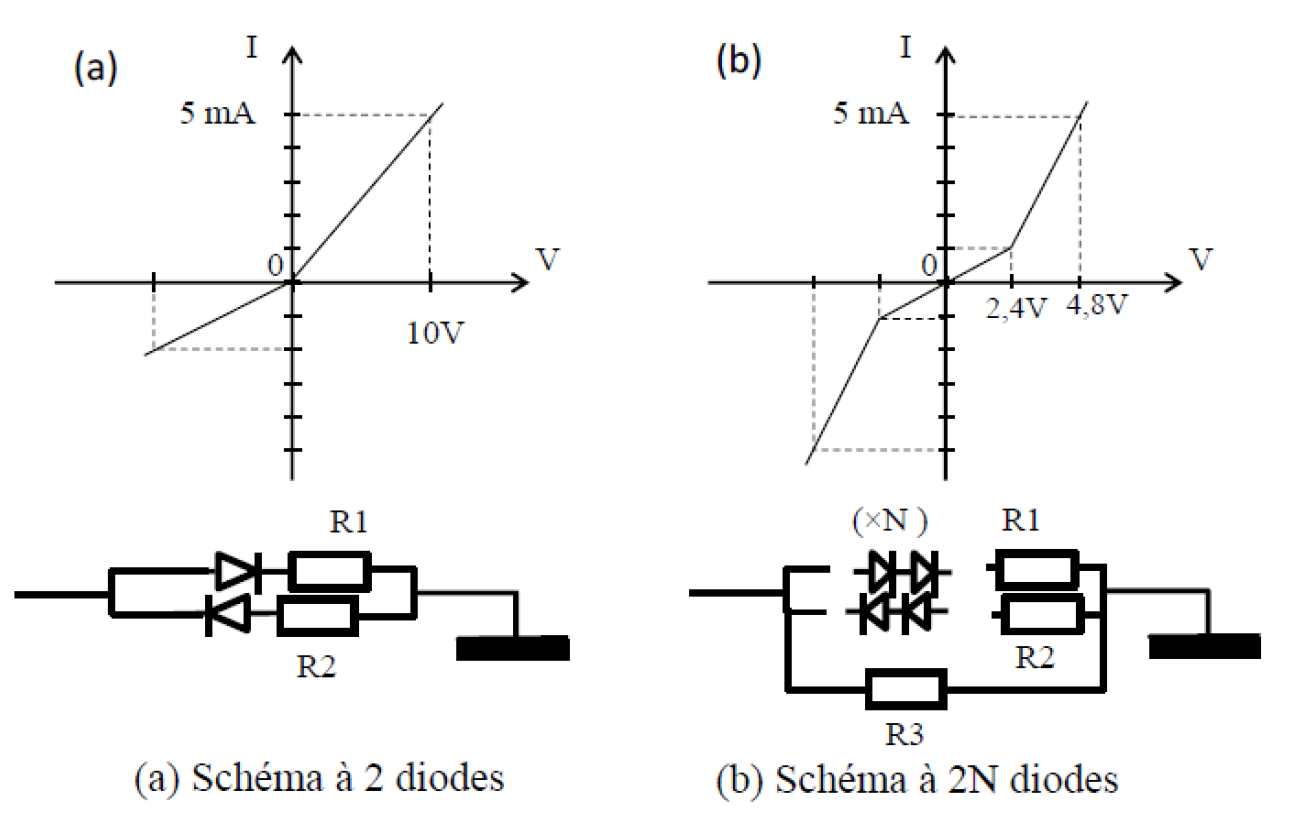
\includegraphics[width=12cm]{images/diodes_002_a.png}
\end{center}

\begin{enumerate}
	\item Dans le cas du montage de la figure (a) et d'utilisation de diodes parfaites et idéales, que doivent valoir $R_1$ et $R_2$ pour obtenir la caractéristique tracée dans le graphe $I(V)$ ?
	\item Dans le cas du montage de la figure (b), les diodes ont pour seuil $0,6\operatorname{V}$. Que doivent valoir $R_1$, $R_2$ et $R_3$ et le nombre de diodes $N$ ($N = 2$ a été dessiné arbitrairement) pour obtenir la caractéristique tracée dans le graphe $I(V)$ ?
\end{enumerate}
}

%%%%%%%%%%%%%%%%%%%
%%%%%%%%%%%%%%%%%%%
\encadreTDExo{4.B1 - Emettre des photons à partir d'une LED}{

On souhaite réaliser un montage émetteur à l'aide d'une \textbf{diode rouge} de type KingBright L-53HD. On propose d'étudier le montage suivant :

\begin{center}
	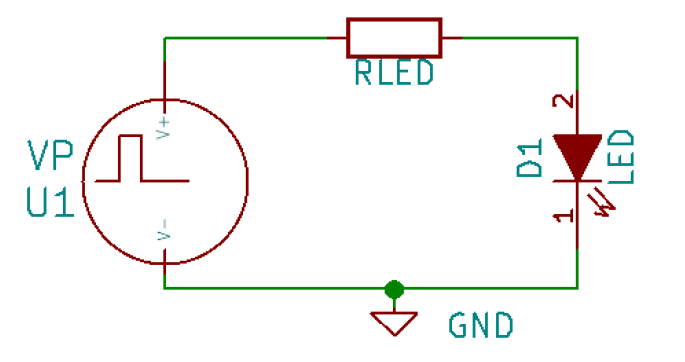
\includegraphics[width=8cm]{images/emetteur_003_a.png}
\end{center}

On donne une partie de la documentation : 

\begin{center}
	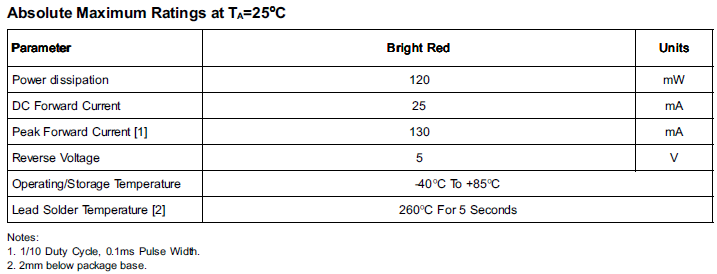
\includegraphics[width=14cm]{images/doc_led_rouge.png}
\end{center}


\begin{enumerate}
	\item Cas 1 : La source de tension $V_P$ est une \textbf{source continue}. Elle délivre une différence de potentiel de $5\operatorname{V}$.
	\begin{enumerate}
		\item Quelle est la valeur maximale du courant que la diode peut supporter dans ces conditions ?
		\item Quelle est la valeur minimale que doit avoir $R_{LED}$ pour respecter cette condition ?
		\item Quel sera alors le courant moyen qui traversera la LED ?
	\end{enumerate}
	
	\item Cas 2 : La source de tension $V_P$ est une \textbf{source impulsionnelle}. Elle délivre des impulsions de $5\operatorname{V}$ de durée $0.1\operatorname{ms}$ avec une fréquence de répétition de $1\operatorname{kHz}$.
	\begin{enumerate}
		\item Quelle est la valeur maximale du courant que la diode peut supporter dans ces conditions ?
		\item Quelle est la valeur minimale que doit avoir $R_{LED}$ pour respecter cette condition ?
		\item Quel sera alors le courant moyen qui traversera la LED ?
	\end{enumerate}
\end{enumerate}
}


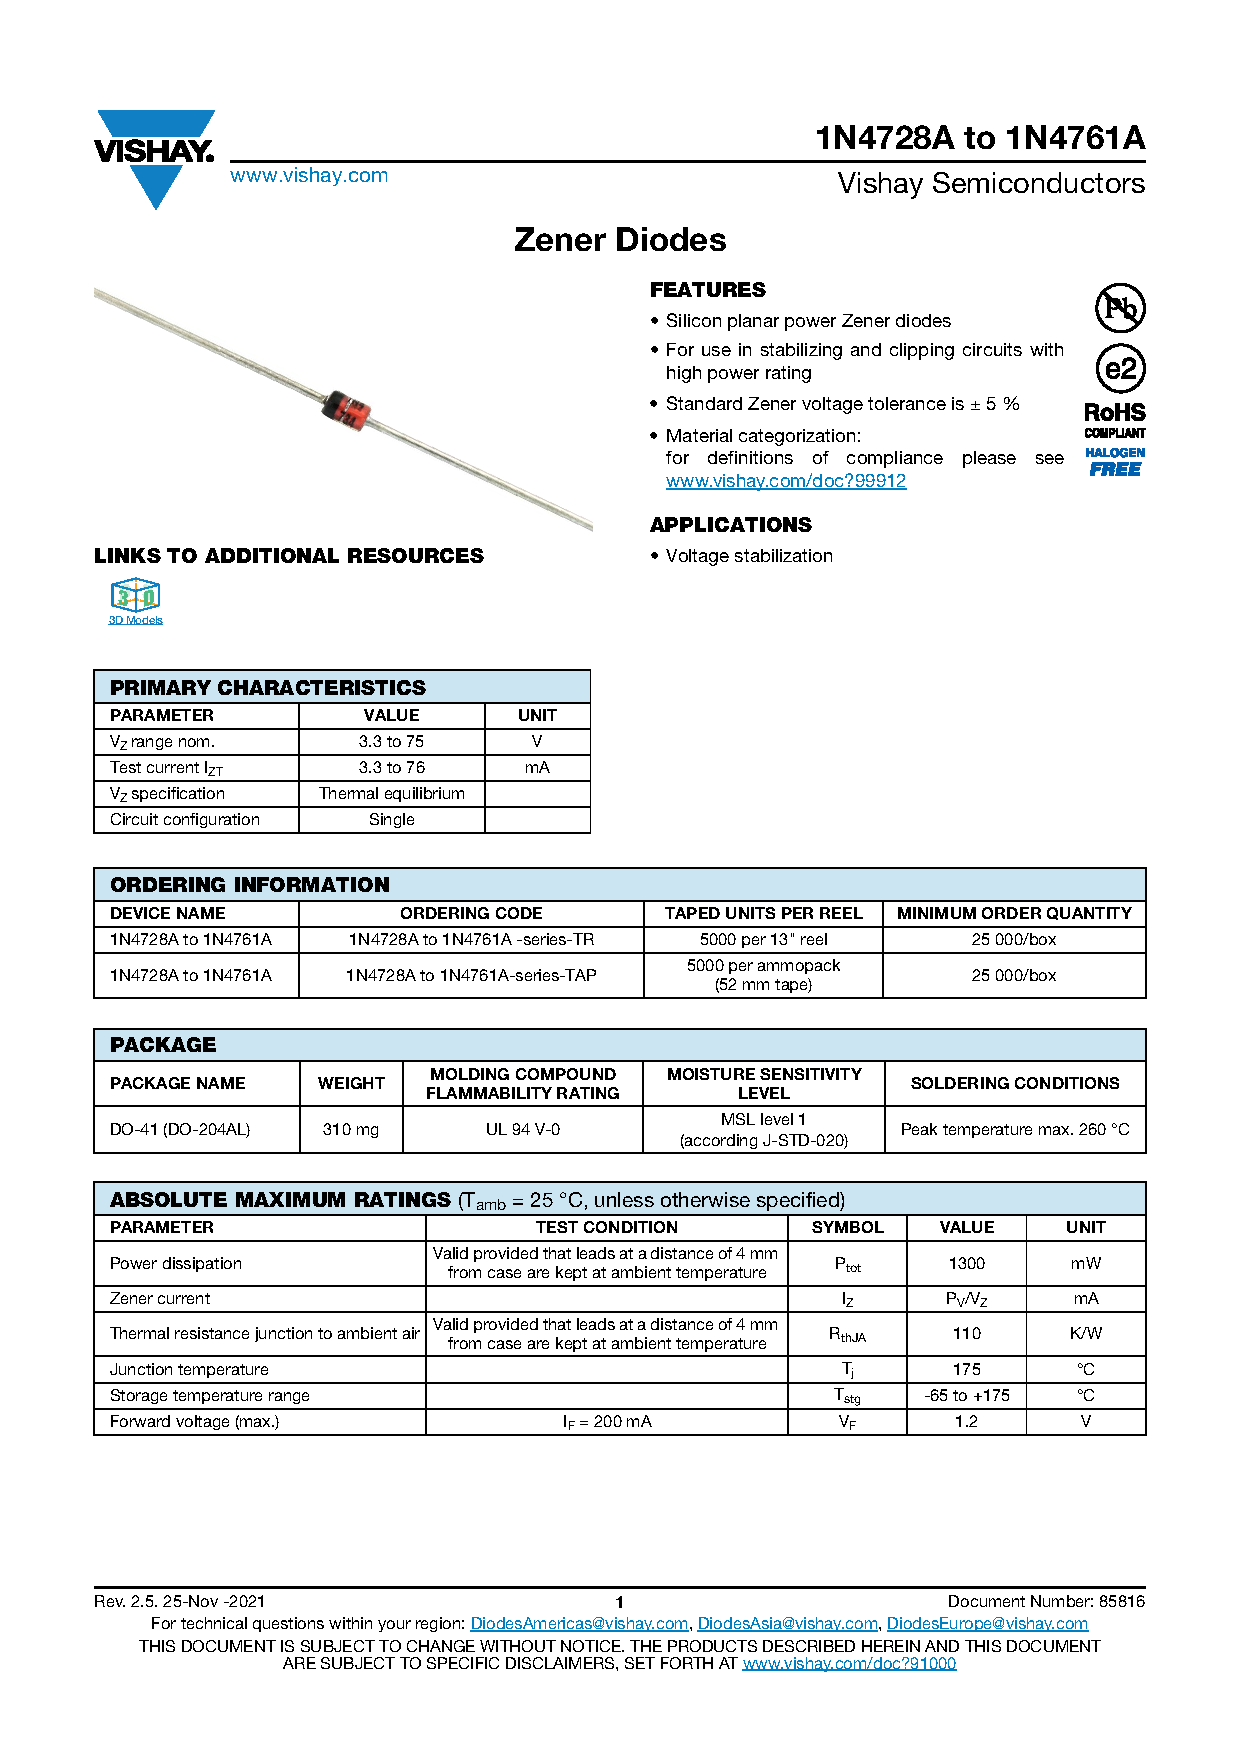
\includepdf[pages=1-2]{docs/1n4728a.pdf}

\end {document}